\documentclass[tikz, border=10pt]{standalone}

\usepackage{xcolor}
\definecolor{jgurot}{RGB}{193,0,42}
\definecolor{jguhgrau}{RGB}{172,172,172}
\definecolor{jgudgrau}{RGB}{99,99,99}

\begin{document}
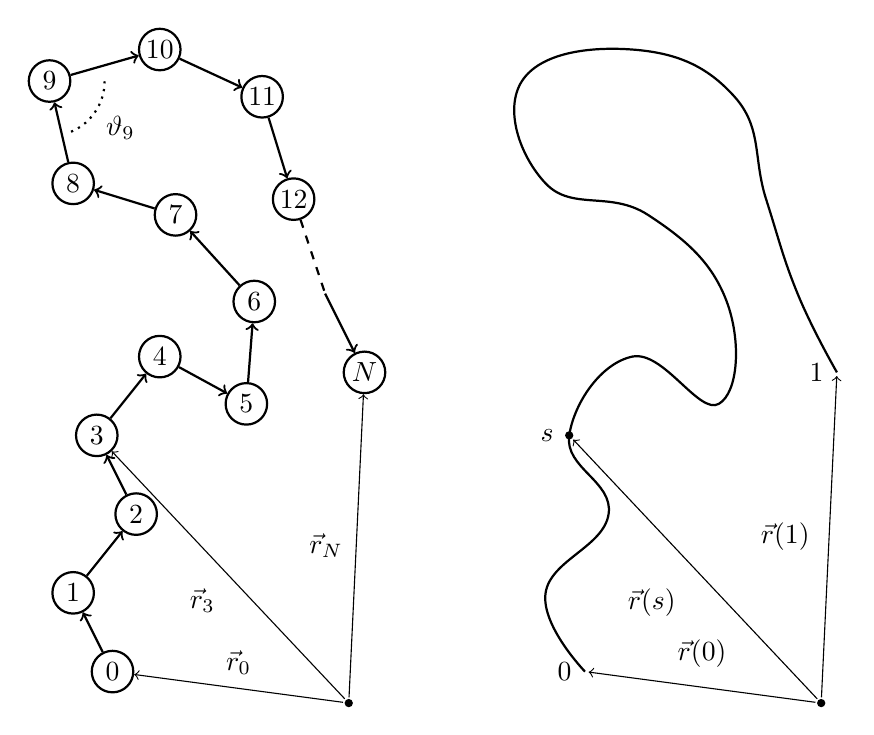
\begin{tikzpicture}[
  rotate=90,
  knoten/.style={
    shape=circle,
    inner sep=0pt,
    minimum size=1.5em,
    thick
  },
  dot/.style={
    draw=none, scale=0.2, shape=circle, fill=black, minimum size=1.5em, outer sep=3pt
  }
]

\draw (0, 0-0.5) node [knoten,draw] (n0) {$0$};
\draw (1, 0.5-0.5) node [knoten,draw] (n1) {$1$};
\draw (2, -0.3-0.5) node [knoten,draw] (n2) {$2$};
\draw (3, 0.2-0.5) node [knoten,draw] (n3) {$3$};
\draw (4, -0.6-0.5) node [knoten,draw] (n4) {$4$};
\draw (3.4, -1.7-0.5) node [knoten,draw] (n5) {$5$};
\draw (4.7, -2.3) node [knoten,draw] (n6) {$6$};
\draw (5.8, -1.3) node [knoten,draw] (n7) {$7$};
\draw (6.2, 0.0) node [knoten,draw] (n8) {$8$};
\draw (7.5, 0.3) node [knoten,draw] (n9) {$9$};
\draw (7.9, -1.1) node [knoten,draw] (n10) {$10$};
\draw (7.3, -2.4) node [knoten,draw] (n11) {$11$};
\draw (6.0, -2.8) node [knoten,draw] (n12) {$12$};
\draw (4.8, -3.2) node [outer sep=0pt, inner sep=0pt, minimum size=0pt] (n13) {};
\draw (3.8, -3.7) node [knoten,draw] (nN) {$N$};

% \draw[Darkgreen,thick] (n9) arc (90:180:1cm);
\draw[thick,dotted] ([shift=(203:0.7cm)]7.5,0.3) arc (203:275:0.7cm);
\draw[] (6.9,-0.6) node {$\vartheta_9$};
% \draw [red,thick,domain=0:90] plot (7.5, 0.3)+({cos(\x)}, {sin(\x)});

\draw (-0.4, -3.5) node [dot] (O) {};

% \draw (-0.4, -3.5) node [dot] (O) {};
% \draw (0, 0-0.5) node [label=below left:$0$] (0) {};
% \draw (3.8, -3.7) node [label=left:$1$] (1) {};
% \draw (3, 0.2-0.5) node [dot,label=left:$s$] (s) {};

\path
  (O) edge [->] node [outer sep=-2pt,label=above:$\vec r_0$] {}  (n0)
  (O) edge [->] node [outer sep=-2pt,label=below left:$\vec r_3$] {}  (n3)
  (O) edge [->] node [outer sep=-2pt,label=left:$\vec r_N$] {}  (nN)
  ;

\path [thick]
      (n0) edge[->] (n1)
      (n1) edge[->] (n2)
      (n2) edge[->] (n3)
      (n3) edge[->] (n4)
      (n4) edge[->] (n5)
      (n5) edge[->] (n6)
      (n6) edge[->] (n7)
      (n7) edge[->] (n8)
      (n8) edge[->] (n9)
      (n9) edge[->] (n10)
      (n10) edge[->] (n11)
      (n11) edge[->] (n12)
      (n12) edge[dashed] (n13)
      (n13) edge[->] (nN);

      % gauss
      \draw (-0.4, -3.5 - 6) node [dot] (rO) {};
      \draw (0, 0-0.5 - 6) node [outer sep=-2pt,label=left:$0$] (0) {};
      \draw (3.8, -3.7 - 6) node [outer sep=-2pt,label=left:$1$] (1) {};
      \draw (3, 0.2-0.5 - 6) node [outer sep=-2pt,dot,label=left:$s$] (s) {};

      \path
        (rO) edge [->] node [label=above:$\vec r(0)$] {}  (0)
        (rO) edge [->] node [label=below left:$\vec r(s)$] {}  (s)
        (rO) edge [->] node [label=left:$\vec r(1)$] {}  (1)
        ;

      \draw [thick] plot [smooth, tension=0.75]
            coordinates {
              (0, 0-0.5 - 6)
              (1, 0.5-0.5 - 6)
              (2, -0.3-0.5 - 6)
              (3, 0.2-0.5 - 6)
              (4, -0.6-0.5 - 6)
              (3.4, -1.7-0.5 - 6)
              (4.7, -2.3 - 6)
              (5.8, -1.3 - 6)
              (6.2, 0.0 - 6)
              (7.5, 0.3 - 6)
              (7.9, -1.1 - 6)
              (7.3, -2.4 - 6)
              (6.0, -2.8 - 6)
              (4.8, -3.2 - 6)
              (3.8, -3.7 - 6)
            };
\end{tikzpicture}
\end{document}
